\techsection{FRONT VIEW}
\vspace{-0.3cm}

\begin{tabular}{p{0.49\textwidth}|p{0.49\textwidth}}
% Left side
\begin{center}
\begin{tikzpicture}
\node[draw=bordercolor, line width=1pt, inner sep=4pt, fill=white, rounded corners=2pt] {
    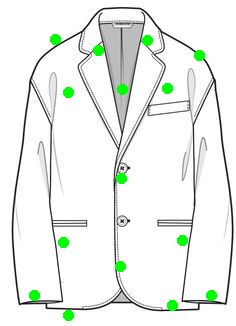
\includegraphics[width=0.35\textwidth,height=12cm,keepaspectratio]{blazer_illustration_front.png}
};
\end{tikzpicture}
\end{center}
&
% Right side - Attributes Table 
\specificationtable{
Component & Specification \\  
1 & The collar and lapel area should be carefully shaped with sturdy interfacing to maintain structure \\  
2 & Top center neckline finished cleanly, ensuring smooth back neck facing \\  
3 & Right bottom hem corner reinforced and aligned with side seam for durability \\  
4 & Left bottom hem corner balanced with the front panels and similarly reinforced \\  
5 & Upper button placement area to include interfacing for extra support \\  
6 & Main closure button region securely stitched and properly spaced \\  
7 & Chest pocket welt shaped neatly and symmetrically to the lapel line \\  
8 & Side seam at waist pocket finished with neat edge and continuous panel alignment \\  
9 & Right waist pocket opening placed level and properly reinforced inside \\  
10 & Left shoulder seam slightly padded to preserve crisp silhouette \\  
11 & Right shoulder seam designed to match left side with equal slope and padding \\  
}
\end{tabular}

\vspace{0.5cm}

% MEASUREMENTS TABLE
\measurementtable{
Keypoint & Measurement & Value & Tolerance & Method & Reference & Comments \\  
1 & Collar/ Lapel Depth & 4 cm & ±0.3 cm & Measure from fold to edge & top collar & - \\  
2 & Neck Width & 15 cm & ±0.5 cm & Across the back neckline & seam-to-seam & - \\  
3 & Right Hem Length & 72 cm & ±1 cm & HPS to bottom edge (right) & front panel & - \\  
4 & Left Hem Length & 72 cm & ±1 cm & HPS to bottom edge (left) & front panel & - \\  
5 & Upper Button Position & 45 cm & ±0.5 cm & From neck seam to first button & vertical center & - \\  
6 & Button Spacing & 10 cm & ±0.3 cm & Between front closure buttons & along center & - \\  
7 & Chest Pocket Height & 12 cm & ±0.5 cm & Pocket opening from side seam & measure horizontally & - \\  
8 & Side Seam Length & 40 cm & ±1 cm & From armhole to hem & along side seam & - \\  
9 & Waist Pocket Width & 14 cm & ±0.5 cm & Horizontal pocket opening & measure edge-to-edge & - \\  
10 & Shoulder Seam (Left) & 14 cm & ±0.5 cm & Collar junction to sleeve cap & left side & - \\  
11 & Shoulder Seam (Right) & 14 cm & ±0.5 cm & Collar junction to sleeve cap & right side & - \\  
}

\techsection{BACK VIEW}
\vspace{-0.3cm}

\begin{tabular}{p{0.49\textwidth}|p{0.49\textwidth}}
% Left side
\begin{center}
\begin{tikzpicture}
\node[draw=bordercolor, line width=1pt, inner sep=4pt, fill=white, rounded corners=2pt] {
    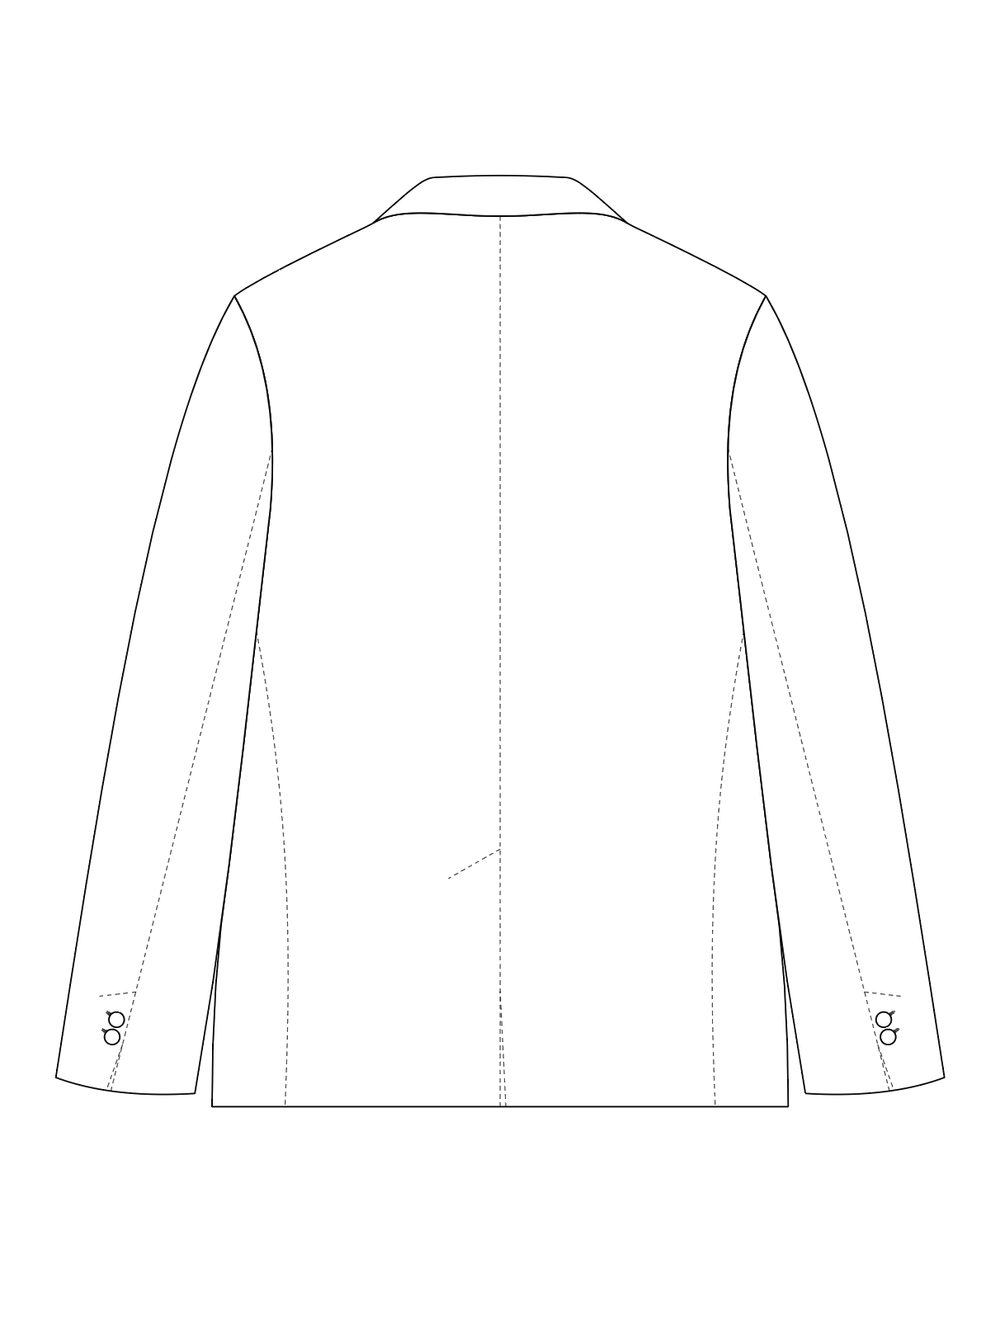
\includegraphics[width=0.35\textwidth,height=12cm,keepaspectratio]{blazer_illustration_back.png}
};
\end{tikzpicture}
\end{center}
&
% Right side - Attributes Table 
\specificationtable{
Component & Specification \\  
1 & Center back neckline area shaped with a smooth seam and reinforced collar join \\  
2 & Right cuff edge finished with a clean hem and button vent \\  
3 & Left cuff edge similarly finished with matching vent detail \\  
4 & Right hem corner tapered to follow the jacket silhouette and reinforced \\  
5 & Left elbow section shaped for mobility with adequate ease \\  
6 & Right elbow seam allowance pressed open for a smooth finish, matching the left \\  
7 & Left side seam aligned with the back panel for proper drape \\  
8 & Right shoulder seam contoured to follow shoulder slope \\  
9 & Left shoulder seam balanced with right side for symmetrical fit \\  
}
\end{tabular}

\vspace{0.5cm}

% MEASUREMENTS TABLE
\measurementtable{
Keypoint & Measurement & Value & Tolerance & Method & Reference & Comments \\  
1 & Back Neck Width & 16 cm & ±0.5 cm & Seam-to-seam across neck & top back & - \\  
2 & Right Sleeve Cuff Opening & 13 cm & ±0.5 cm & Circumference at cuff & right sleeve & - \\  
3 & Left Sleeve Cuff Opening & 13 cm & ±0.5 cm & Circumference at cuff & left sleeve & - \\  
4 & Right Hem to Shoulder & 75 cm & ±1 cm & From hem corner vertically to shoulder & center back & - \\  
5 & Left Elbow Width & 18 cm & ±0.8 cm & Around elbow area & left sleeve & - \\  
6 & Right Elbow Width & 18 cm & ±0.8 cm & Around elbow area & right sleeve & - \\  
7 & Side Seam Length (Left) & 42 cm & ±1 cm & Armhole to hem & along side & - \\  
8 & Shoulder Slope (Right) & 15° & ±1° & Measure angle at shoulder line & right side & - \\  
9 & Shoulder Slope (Left) & 15° & ±1° & Measure angle at shoulder line & left side & - \\  
}